% Options for packages loaded elsewhere
\PassOptionsToPackage{unicode}{hyperref}
\PassOptionsToPackage{hyphens}{url}
%
\documentclass[
]{article}
\usepackage{lmodern}
\usepackage{amssymb,amsmath}
\usepackage{ifxetex,ifluatex}
\ifnum 0\ifxetex 1\fi\ifluatex 1\fi=0 % if pdftex
  \usepackage[T1]{fontenc}
  \usepackage[utf8]{inputenc}
  \usepackage{textcomp} % provide euro and other symbols
\else % if luatex or xetex
  \usepackage{unicode-math}
  \defaultfontfeatures{Scale=MatchLowercase}
  \defaultfontfeatures[\rmfamily]{Ligatures=TeX,Scale=1}
\fi
% Use upquote if available, for straight quotes in verbatim environments
\IfFileExists{upquote.sty}{\usepackage{upquote}}{}
\IfFileExists{microtype.sty}{% use microtype if available
  \usepackage[]{microtype}
  \UseMicrotypeSet[protrusion]{basicmath} % disable protrusion for tt fonts
}{}
\makeatletter
\@ifundefined{KOMAClassName}{% if non-KOMA class
  \IfFileExists{parskip.sty}{%
    \usepackage{parskip}
  }{% else
    \setlength{\parindent}{0pt}
    \setlength{\parskip}{6pt plus 2pt minus 1pt}}
}{% if KOMA class
  \KOMAoptions{parskip=half}}
\makeatother
\usepackage{xcolor}
\IfFileExists{xurl.sty}{\usepackage{xurl}}{} % add URL line breaks if available
\IfFileExists{bookmark.sty}{\usepackage{bookmark}}{\usepackage{hyperref}}
\hypersetup{
  pdftitle={EpiMod: Lotka-Volterra},
  pdfauthor={Beccuti Marco, Castagno Paolo, Pernice Simone},
  hidelinks,
  pdfcreator={LaTeX via pandoc}}
\urlstyle{same} % disable monospaced font for URLs
\usepackage[margin=1in]{geometry}
\usepackage{color}
\usepackage{fancyvrb}
\newcommand{\VerbBar}{|}
\newcommand{\VERB}{\Verb[commandchars=\\\{\}]}
\DefineVerbatimEnvironment{Highlighting}{Verbatim}{commandchars=\\\{\}}
% Add ',fontsize=\small' for more characters per line
\usepackage{framed}
\definecolor{shadecolor}{RGB}{248,248,248}
\newenvironment{Shaded}{\begin{snugshade}}{\end{snugshade}}
\newcommand{\AlertTok}[1]{\textcolor[rgb]{0.94,0.16,0.16}{#1}}
\newcommand{\AnnotationTok}[1]{\textcolor[rgb]{0.56,0.35,0.01}{\textbf{\textit{#1}}}}
\newcommand{\AttributeTok}[1]{\textcolor[rgb]{0.77,0.63,0.00}{#1}}
\newcommand{\BaseNTok}[1]{\textcolor[rgb]{0.00,0.00,0.81}{#1}}
\newcommand{\BuiltInTok}[1]{#1}
\newcommand{\CharTok}[1]{\textcolor[rgb]{0.31,0.60,0.02}{#1}}
\newcommand{\CommentTok}[1]{\textcolor[rgb]{0.56,0.35,0.01}{\textit{#1}}}
\newcommand{\CommentVarTok}[1]{\textcolor[rgb]{0.56,0.35,0.01}{\textbf{\textit{#1}}}}
\newcommand{\ConstantTok}[1]{\textcolor[rgb]{0.00,0.00,0.00}{#1}}
\newcommand{\ControlFlowTok}[1]{\textcolor[rgb]{0.13,0.29,0.53}{\textbf{#1}}}
\newcommand{\DataTypeTok}[1]{\textcolor[rgb]{0.13,0.29,0.53}{#1}}
\newcommand{\DecValTok}[1]{\textcolor[rgb]{0.00,0.00,0.81}{#1}}
\newcommand{\DocumentationTok}[1]{\textcolor[rgb]{0.56,0.35,0.01}{\textbf{\textit{#1}}}}
\newcommand{\ErrorTok}[1]{\textcolor[rgb]{0.64,0.00,0.00}{\textbf{#1}}}
\newcommand{\ExtensionTok}[1]{#1}
\newcommand{\FloatTok}[1]{\textcolor[rgb]{0.00,0.00,0.81}{#1}}
\newcommand{\FunctionTok}[1]{\textcolor[rgb]{0.00,0.00,0.00}{#1}}
\newcommand{\ImportTok}[1]{#1}
\newcommand{\InformationTok}[1]{\textcolor[rgb]{0.56,0.35,0.01}{\textbf{\textit{#1}}}}
\newcommand{\KeywordTok}[1]{\textcolor[rgb]{0.13,0.29,0.53}{\textbf{#1}}}
\newcommand{\NormalTok}[1]{#1}
\newcommand{\OperatorTok}[1]{\textcolor[rgb]{0.81,0.36,0.00}{\textbf{#1}}}
\newcommand{\OtherTok}[1]{\textcolor[rgb]{0.56,0.35,0.01}{#1}}
\newcommand{\PreprocessorTok}[1]{\textcolor[rgb]{0.56,0.35,0.01}{\textit{#1}}}
\newcommand{\RegionMarkerTok}[1]{#1}
\newcommand{\SpecialCharTok}[1]{\textcolor[rgb]{0.00,0.00,0.00}{#1}}
\newcommand{\SpecialStringTok}[1]{\textcolor[rgb]{0.31,0.60,0.02}{#1}}
\newcommand{\StringTok}[1]{\textcolor[rgb]{0.31,0.60,0.02}{#1}}
\newcommand{\VariableTok}[1]{\textcolor[rgb]{0.00,0.00,0.00}{#1}}
\newcommand{\VerbatimStringTok}[1]{\textcolor[rgb]{0.31,0.60,0.02}{#1}}
\newcommand{\WarningTok}[1]{\textcolor[rgb]{0.56,0.35,0.01}{\textbf{\textit{#1}}}}
\usepackage{graphicx,grffile}
\makeatletter
\def\maxwidth{\ifdim\Gin@nat@width>\linewidth\linewidth\else\Gin@nat@width\fi}
\def\maxheight{\ifdim\Gin@nat@height>\textheight\textheight\else\Gin@nat@height\fi}
\makeatother
% Scale images if necessary, so that they will not overflow the page
% margins by default, and it is still possible to overwrite the defaults
% using explicit options in \includegraphics[width, height, ...]{}
\setkeys{Gin}{width=\maxwidth,height=\maxheight,keepaspectratio}
% Set default figure placement to htbp
\makeatletter
\def\fps@figure{htbp}
\makeatother
\setlength{\emergencystretch}{3em} % prevent overfull lines
\providecommand{\tightlist}{%
  \setlength{\itemsep}{0pt}\setlength{\parskip}{0pt}}
\setcounter{secnumdepth}{-\maxdimen} % remove section numbering
\usepackage{float} \usepackage{url} \usepackage{booktabs} \usepackage{multirow} \floatplacement{figure}{H} \usepackage{caption} \captionsetup[table]{skip=10pt}

\title{EpiMod: Lotka-Volterra}
\author{Beccuti Marco, Castagno Paolo, Pernice Simone}
\date{}

\begin{document}
\maketitle

{
\setcounter{tocdepth}{3}
\tableofcontents
}
\hypertarget{the-lotkavolterra-model}{%
\subsection{The Lotka--Volterra model}\label{the-lotkavolterra-model}}

The Lotka--Volterra equations, also known as the predator--prey
equations, are a pair of first-order nonlinear differential equations,
frequently used to describe the dynamics of biological systems in which
two species interact, one as a predator and the other as prey. The
populations change through time according to the pair of equations:

\begin{figure}
\centering
\includegraphics{https://render.githubusercontent.com/render/math?math=\%5Cbegin\%7Balign\%7D\%20\%20\%20\%5Cfrac\%7Bdx\%7D\%7Bdt\%7D\%20\%26\%3D\%20\%5Calpha\%20x-\%5Cbeta\%20xy\%2C\%5C\%5C\%20\%20\%20\%5Cfrac\%7Bdy\%7D\%7Bdt\%7D\%20\%26\%3D\%20\%5Cdelta\%20xy-\%5Cgamma\%20y\%2C\%20\%20\%5Cnonumber\%20\%5Cend\%7Balign\%7D}
\caption{\begin{align}   \frac{dx}{dt} &= \alpha x-\beta xy,\\   \frac{dy}{dt} &= \delta xy-\gamma y,  \nonumber \end{align}}
\end{figure}

where:

\begin{enumerate}
\def\labelenumi{\arabic{enumi}.}
\tightlist
\item
  \(x\) is the number of prey (for example, rabbits);
\item
  \(y\) is the number of some predator (for example, foxes);
\item
  \(\frac{dy}{dt}\) and \(\frac{dx}{dt}\) represent the instantaneous
  growth rates of the two populations;
\item
  \(t\) represents time;
\item
  \(\alpha,\ \beta,\ \gamma,\ \theta\) are positive real parameters
  describing the interaction of the two species.
\end{enumerate}

\hypertarget{starting}{%
\subsection{Starting}\label{starting}}

\begin{Shaded}
\begin{Highlighting}[]
\KeywordTok{library}\NormalTok{(epimod)}
\end{Highlighting}
\end{Shaded}

Download all the docker images used by \emph{epimod}:

\begin{Shaded}
\begin{Highlighting}[]
\KeywordTok{downloadContainers}\NormalTok{()}
\end{Highlighting}
\end{Shaded}

\hypertarget{model-generation}{%
\subsection{Model generation}\label{model-generation}}

\begin{Shaded}
\begin{Highlighting}[]

\KeywordTok{model_generation}\NormalTok{(}\DataTypeTok{net_fname =} \StringTok{"./Net/Lotka-Volterra.PNPRO"}\NormalTok{)}
\end{Highlighting}
\end{Shaded}

\hypertarget{sensitivity-analysis}{%
\subsubsection{Sensitivity analysis}\label{sensitivity-analysis}}

The R function \emph{sensitivity\_analysis()} implements the sensitivity
analysis taking as input

\begin{enumerate}
\def\labelenumi{\arabic{enumi}.}
\tightlist
\item
  the \emph{.solver} file generated by the \emph{model\_generation}
  function, the total number of samplings to be performed,
\item
  the final solution time,
\item
  the time step defining the frequency at which explicit estimates for
  the system values are desired,
\item
  parameters\_fname (\emph{Functions\_list.csv}): a textual file in
  which the parameters to be studied are listed associated with their
  range of variability. significato delle colonne, e che serve il ; come
  sep, spazi non nei path An example is given by the following file,
  where
\end{enumerate}

\begin{verbatim}
#>   V1    V2               V3                       V4                     V5
#> 1  i  init  init_generation  min_init = c(0.9 , 0.8)  max_init = c(1.8 , 2)
\end{verbatim}

\begin{enumerate}
\def\labelenumi{\arabic{enumi}.}
\setcounter{enumi}{4}
\tightlist
\item
  functions\_fname (\emph{Functions.R}): \ldots{}
\end{enumerate}

\begin{Shaded}
\begin{Highlighting}[]
\NormalTok{init_generation<-}\ControlFlowTok{function}\NormalTok{(min_init , max_init)}
\NormalTok{\{}
    \CommentTok{# min/max are vectors = first position interval values for the first place}
    \CommentTok{# and second position for the second place.}

\NormalTok{   i_}\DecValTok{1}\NormalTok{=}\KeywordTok{runif}\NormalTok{(}\DataTypeTok{n=}\DecValTok{1}\NormalTok{,}\DataTypeTok{min=}\NormalTok{min_init[}\DecValTok{1}\NormalTok{],}\DataTypeTok{max=}\NormalTok{max_init[}\DecValTok{1}\NormalTok{])}
\NormalTok{   i_}\DecValTok{2}\NormalTok{=}\KeywordTok{runif}\NormalTok{(}\DataTypeTok{n=}\DecValTok{1}\NormalTok{,}\DataTypeTok{min=}\NormalTok{min_init[}\DecValTok{2}\NormalTok{],}\DataTypeTok{max=}\NormalTok{max_init[}\DecValTok{2}\NormalTok{])}

   \KeywordTok{return}\NormalTok{( }\KeywordTok{c}\NormalTok{(i_}\DecValTok{1}\NormalTok{,i_}\DecValTok{2}\NormalTok{) )}
\NormalTok{\}}
\end{Highlighting}
\end{Shaded}

\begin{enumerate}
\def\labelenumi{\arabic{enumi}.}
\setcounter{enumi}{5}
\tightlist
\item
  target\_value\_fname (\emph{Target.R}): \ldots{} .
\end{enumerate}

Assuming the following fixed rates: \(\beta = 4/3,\  \theta = 1.\) Than
we change the prey and predator initial conditions from 200 to 1800, and
the prey and predator birth rates \(\alpha,\ \gamma\) from 0.1 to 2,
knowing that we are interested to the trajectory generated with the
following values:
\(x(0) = 1000,\ y(0)=500,\ \alpha = 2/3,\ \gamma = 1\).

\hypertarget{prcc-and-ranking}{%
\paragraph{PRCC and ranking}\label{prcc-and-ranking}}

This step is necessary if we are interested to calculate the PRCC to
identify among the input parameters which are the sensitive ones (i.e.,
those that have a great effect on the model behaviour). This may
simplify the calibration step reducing (1) the number of variables to be
estimated and (2) the search space associated with each estimated
parameter.

In order to run the simulations, the user must provide

\begin{enumerate}
\def\labelenumi{\arabic{enumi}.}
\tightlist
\item
  the reference dataset;
\item
  the definition of a function to compute the distance (or error)
  between the models' output and the reference dataset itself.
\end{enumerate}

In this case the reference dataset is the trajectory obtained from the
starting point 1 predator and 1 prey. Similarly to the previouos step,
we generate different initial conditions for the system but in this
case.

The function defining the distance takes in inputs only the reference
data and the simulation's output (i.e.~a trajectory); an example it
could be the following:

\begin{Shaded}
\begin{Highlighting}[]
\NormalTok{msqd<-}\ControlFlowTok{function}\NormalTok{(reference, output)}
\NormalTok{\{}
\NormalTok{    Predator <-}\StringTok{ }\NormalTok{output[,}\StringTok{"Predator"}\NormalTok{]}
\NormalTok{    Prey <-}\StringTok{ }\NormalTok{output[,}\StringTok{"Prey"}\NormalTok{]}

\NormalTok{    diff.Predator <-}\StringTok{ }\KeywordTok{sum}\NormalTok{(( Predator }\OperatorTok{-}\StringTok{ }\NormalTok{reference[,}\DecValTok{2}\NormalTok{] )}\OperatorTok{^}\DecValTok{2}\NormalTok{ )}
\NormalTok{    diff.Prey <-}\StringTok{ }\KeywordTok{sum}\NormalTok{(( Prey }\OperatorTok{-}\StringTok{ }\NormalTok{reference[,}\DecValTok{1}\NormalTok{] )}\OperatorTok{^}\DecValTok{2}\NormalTok{ )}

    \KeywordTok{return}\NormalTok{(diff.Predator}\OperatorTok{+}\NormalTok{diff.Prey)}
\NormalTok{\}}
\end{Highlighting}
\end{Shaded}

where the squared error between the Predator and Prey trajectories
obtaained from the simulation and the corresponding reference
trajectories are calculated, respectively named \emph{diff.Predator} and
\emph{diff.Prey}. Then, the sum of these errors is returned. Our purpose
will be to minimize (see next section) this function in order to
identify the trajectory most similar to the reference data, therefore

\begin{Shaded}
\begin{Highlighting}[]
\NormalTok{Target<-}\ControlFlowTok{function}\NormalTok{(output)}
\NormalTok{\{}
\NormalTok{    ret <-}\StringTok{ }\NormalTok{output[,}\StringTok{"Predator"}\NormalTok{]}
    \KeywordTok{return}\NormalTok{(}\KeywordTok{as.data.frame}\NormalTok{(ret))}
\NormalTok{\}}
\end{Highlighting}
\end{Shaded}

Let us note that the name of the distance and target function must have
the same name of the corresponding R file.

\begin{Shaded}
\begin{Highlighting}[]

\NormalTok{sensitivity<-}\KeywordTok{sensitivity_analysis}\NormalTok{(}\DataTypeTok{n_config =} \DecValTok{30}\NormalTok{,}
                                  \DataTypeTok{parameters_fname =} \StringTok{"Input/Functions_list.csv"}\NormalTok{,}
                                  \DataTypeTok{functions_fname =} \StringTok{"Rfunction/Functions.R"}\NormalTok{,}
                                  \DataTypeTok{solver_fname =} \StringTok{"Net/Lotka-Volterra.solver"}\NormalTok{,}
                                  \DataTypeTok{reference_data =} \StringTok{"Input/reference_data.csv"}\NormalTok{,}
                                  \DataTypeTok{distance_measure_fname =} \StringTok{"Rfunction/msqd.R"}\NormalTok{ ,}
                                  \DataTypeTok{target_value_fname =} \StringTok{"Rfunction/Target.R"}\NormalTok{ ,}
                                  \DataTypeTok{parallel_processors =} \DecValTok{2}\NormalTok{,}
                                  \DataTypeTok{f_time =} \DecValTok{20}\NormalTok{,}
                                  \DataTypeTok{s_time =} \FloatTok{.1}\NormalTok{)}
\end{Highlighting}
\end{Shaded}

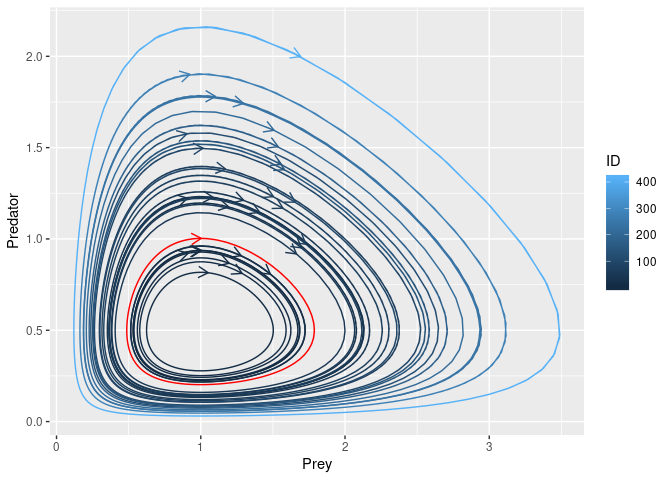
\includegraphics{ReadMe_files/figure-latex/unnamed-chunk-10-1.pdf}

\begin{figure}
\centering
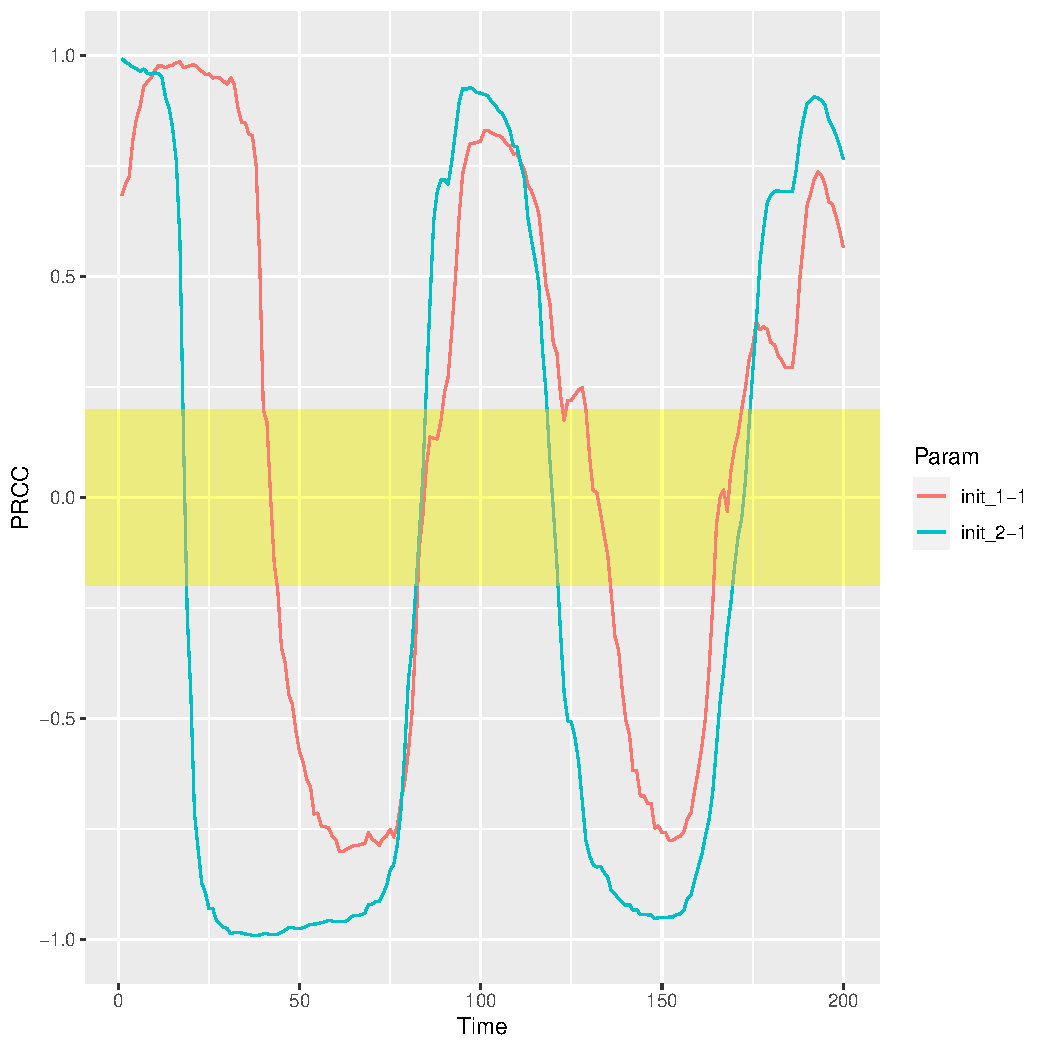
\includegraphics{./Results/results_sensitivity_analysis/prcc_Lotka-Volterra-sensitivity.pdf}
\caption{PRCC for the \textbf{Predator} place over time.}
\end{figure}

Running the sensisitivity analysis, we can replicate the results
reported on Wikipedia,
\emph{\url{https://en.wikipedia.org/wiki/Lotka\%E2\%80\%93Volterra_equations}}.
Indeed, textual file for each generated parameter combination (i.e.~20)
containing the system solution is returned. Each file is characterized
by as many rows as the solution time points (obtained dividing the final
time point by the time step) and as many columns as the system
components. We can now generate the phase-space plot, where it is
possible to see that the predators thrive when there are plentiful prey
but, ultimately, outstrip their food supply and decline. As the predator
population is low, the prey population will increase again. These
dynamics continue in a cycle of growth and decline.

Let us note that it is possible to run the sensitivity analysys without
PRCC or ranking, in the case that we are intersted only on to have a
general idea of the simulation' results.

\hypertarget{calibration-analysis}{%
\subsubsection{Calibration analysis}\label{calibration-analysis}}

\begin{Shaded}
\begin{Highlighting}[]

\KeywordTok{model_calibration}\NormalTok{(}\DataTypeTok{solver_fname =} \StringTok{"Net/Lotka-Volterra.solver"}\NormalTok{,}
                  \DataTypeTok{reference_data =} \StringTok{"Input/reference_data.csv"}\NormalTok{,}
                  \DataTypeTok{distance_measure_fname =} \StringTok{"Rfunction/msqd.R"}\NormalTok{ ,}
                  \DataTypeTok{f_time =} \DecValTok{20}\NormalTok{,}
                  \DataTypeTok{s_time =} \FloatTok{.1}\NormalTok{,}
                  \CommentTok{# Vectors to control the optimization}
                  \DataTypeTok{ini_v =} \KeywordTok{c}\NormalTok{(}\DecValTok{5}\NormalTok{,}\DecValTok{5}\NormalTok{),}
                  \DataTypeTok{ub_v =} \KeywordTok{c}\NormalTok{(}\DecValTok{10}\NormalTok{, }\DecValTok{10}\NormalTok{),}
                  \DataTypeTok{lb_v =} \KeywordTok{c}\NormalTok{(}\DecValTok{0}\NormalTok{, }\DecValTok{0}\NormalTok{),}
                  \DataTypeTok{optim_vector_mod =} \OtherTok{TRUE}\NormalTok{,}
                  \DataTypeTok{max.time =} \DecValTok{60} \CommentTok{# seconds}
\NormalTok{)}
\end{Highlighting}
\end{Shaded}

\hypertarget{whatif-analysis}{%
\subsubsection{Whatif Analysis}\label{whatif-analysis}}

\end{document}
